
\documentclass[letterpaper,11pt]{article}

\usepackage{latexsym}
\usepackage[fleqn]{amsmath}
\usepackage{amssymb}
\usepackage{unicode-math}
\usepackage{fancyhdr}
\usepackage[margin=1.0in, left=0.5in, right=0.5in, top=1.25in, headsep=10mm, headheight=15mm]{geometry}
\usepackage{graphicx}

\setmainfont{Latin Modern Roman}
\setmathfont{Latin Modern Math}

\pagestyle{fancy}
\rhead{Mech 222 Mathematics Worksheets\\ Lecture 7, 8}


\newcommand*\limitset[1]{{#1}^\prime}
% Not working in unicode math with xelatex for some reason...
% \newcommand*\closure[1]{\overline #1}
\newcommand*\closureunion[1]{{#1}\cup \limitset{#1}}
\newcommand*\interior[1]{{#1}^\circ}

% Sets of points
% The set of points within some distance #1 from #2
\newcommand*\neighbor[2]{N_{#1}({#2})}
% The neighborhood without #2
\newcommand*\delneighbor[2]{N_{#1}^*({#2})}
\newcommand*\set[1]{\{ #1 \} }
\newcommand*\conjugate[1]{\overline{#1}}
\newcommand*\sequence[2]{\set{#1}_{#2=1}^\infty}
\newcommand*\series[2]{\sum_{#2=1}^\infty #1_{#2}}
\newcommand*\compose[2]{#1 \circ #2}
\newcommand*\udisk{\mathbb{D}}
\newcommand*\disk[2]{D_{#1}(#2)}
\newcommand*\punctdisk[2]{\disk_{ #1 } - \set{#2}}
\newcommand*\complex{\mathbb{C}}
\newcommand*\naturals{\mathbb{N}}
\newcommand{\integers}{\mathbb{Z}}
\newcommand*\rationals{\mathbb{Q}}
\newcommand*\reals{\mathbb{R}}

% Function spaces
\newcommand*\cnfunc[2]{C^{#2}\left(#1 \right)}
\newcommand*\cnfuncdom[1]{C^{#1}\left(\domain \right)}
\newcommand*\linffunc[1]{L^{\infty}\left(#1 \right)}
\newcommand*\linffuncdom{L^{\infty}\left(\domain \right)}
\newcommand*\lnfunc[2]{L^{#2}\left(#1 \right)}
\newcommand*\lnfuncdom[1]{L^{#1}\left(\domain \right)}
\newcommand*\sobolev[3]{W^{#2, #3}\left(#1 \right)}
\newcommand*\sobolevdom[2]{W^{#1, #2}\left(\domain \right)}
\newcommand*\sobolevh[2]{H^{#2}\left(#1 \right)}
\newcommand*\sobolevhdom[1]{H^{#1}\left(\domain \right)}
\newcommand*\sobolevcs[3]{W_0^{#2, #3}\left(#1 \right)}
\newcommand*\sobolevcsdom[2]{W_0^{#1, #2}\left(\domain \right)}
\newcommand*\sobolevhcs[2]{H_0^{#2}\left(#1 \right)}
\newcommand*\sobolevhcsdom[1]{H_0^{#1}\left(\domain \right)}

\newcommand*\grad{D}
\newcommand*\graddir[1]{D_{#1}}
\newcommand*\lapl{∆}
\newcommand*\diffquot[1]{D^{#1}}
\newcommand*\diffquotdir[2]{D_{#2}^{#1}}

\newcommand*\domain{U}
\newcommand*\bndry[1]{\partial #1}
\newcommand*\bndrydom{\partial \domain}
\newcommand*\compactcont{\subset \subset} % U \compactcont V \rightarrow U \subset \closure{U} \subset V, where U, V are (open) domains

\newcommand*\ballunit{B_1}
\newcommand*\ball[2]{B_{#2}(#1)}
\newcommand*\bunitsurfarea[1]{\omega_{#1}}
\newcommand*\bunitsurfareadef{\omega_n}
\newcommand*\bunitvolume[1]{\alpha_{#1}}
\newcommand*\bunitvolumedef{\alpha_n}

\newcommand*\limitto[2]{\lim \limits_{#1 \rightarrow #2}}

\newcommand{\dd}[1]{\;\mathrm{d}#1}
\newcommand{\dx}{\dd{x}}
\newcommand{\dy}{\dd{y}}
\newcommand{\dz}{\dd{z}}
\newcommand{\dr}{\dd{r}}
\newcommand{\ds}{\dd{s}}
\newcommand{\dS}{\dd{S}}
\newcommand{\dt}{\dd{t}}
\newcommand*\pderiv[2]{\frac{\partial #1}{\partial #2}}
\newcommand*\nthpderiv[3]{\frac{\partial^{#3} #1}{\partial #2^{#3}}}
\newcommand*\deriv[2]{\frac{\dd{#1}}{\dd{#2}}}
\newcommand*\nthderiv[3]{\frac{\dd{^{#3} #1}}{\dd{#2^{#3}}}}

% Norms
\newcommand*\linfnorm[2]{\left\lVert#1\right\rVert_{L^{\infty}(#2)}}
\newcommand*\linfnormdom[1]{\left\lVert#1\right\rVert_{L^{\infty}(\domain)}}

\newcommand*\lnorm[3]{\left\lVert#1\right\rVert_{L^{#2}(#3)}}
\newcommand*\lnormdom[2]{\left\lVert#1\right\rVert_{L^{#2}(\domain)}}

\newcommand*\hnorm[3]{\left\lVert#1\right\rVert_{H^{#2}(#3)}}
\newcommand*\hnormdom[2]{\left\lVert#1\right\rVert_{H^{#2}(\domain)}}

\newcommand*\wnorm[4]{\left\lVert#1\right\rVert_{W^{#2, #3}(#4)}}
\newcommand*\wnormdom[3]{\left\lVert#1\right\rVert_{W^{#2, #3}(\domain)}}

\DeclareMathOperator{\res}{res}
\DeclareMathOperator{\sign}{sign}
\DeclareMathOperator{\diam}{diam}
\DeclareMathOperator{\partition}{Partition}

% Matrix computations
\newcommand*\trace[1]{\text{tr}\left( #1 \right)}

% Average integral from https://tex.stackexchange.com/questions/759/average-integral-symbol
\def\Xint#1{\mathchoice
{\XXint\displaystyle\textstyle{#1}}%
{\XXint\textstyle\scriptstyle{#1}}%
{\XXint\scriptstyle\scriptscriptstyle{#1}}%
{\XXint\scriptscriptstyle\scriptscriptstyle{#1}}%
\!\int}
\def\XXint#1#2#3{{\setbox0=\hbox{$#1{#2#3}{\int}$ }
\vcenter{\hbox{$#2#3$ }}\kern-.6\wd0}}
\def\ddashint{\Xint=}
\def\dashint{\Xint-}
\def\avgint{\dashint}


\begin{document}
\section*{Integration in cylindrical and spherical coordinates}
Similar to how triple integrals are just an extension of double integrals,
cylindrical and spherical coordinates are just extensions of polar coordinates.

Recall the formulas for converting between cartesian coordinates and cylindrical coordinates:
$$
\begin{array}{ccc}
  r^2 = x^2 + y^2     & \theta = \arctan \left( \frac{y}{x} \right) & \hat{z} = z\\
  x = r \cos(\theta) & y = r \sin(\theta)                           & z = \hat{z}
\end{array}
$$
and the conversion between spherical coordinates:
$$
\begin{array}{ccc}
  \rho^2 = x^2 + y^2 + z^2 & \theta = \arctan \left( \frac{y}{x} \right) & \phi = \arctan \left( \frac{z}{\sqrt{x^2 + y^2}} \right)\\
  x = \rho \sin(\phi) \cos(\theta), & y = \rho \sin(\phi) \sin(\theta) & z = \rho \cos(\phi)
\end{array}
$$

The differential element for cylindrical coordinates is just an extrusion of the polar coordinate element.
Then the ``volume'' of the differential element is just
$$\dd{V}_{cylindrical} = \dd{A}_{polar} \dz = r \dr \dd{\theta} \dz$$
\begin{figure*}[h]
  \centering 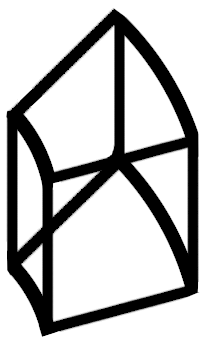
\includegraphics[width=100px]{mech222/worksheet_2b_cylinder_diff_elem.png}
  \caption{Cylindrical coordinates differential area element}
\end{figure*}

The differential element for spherical coordinates is formed by sweeping the polar coordinate area element over a slight rotation.
The volume covered then depends on the angle it starts at and the radius, and the element can be shown to have ``volume''
$$\dd{V}_{spherical} = \rho \sin(\phi) \dd{A}_{polar} \dd{\phi} = \rho^2 \sin(\phi) \dd{\rho} \dd{\theta} \dd{\phi}$$
\begin{figure*}[h]
  \centering 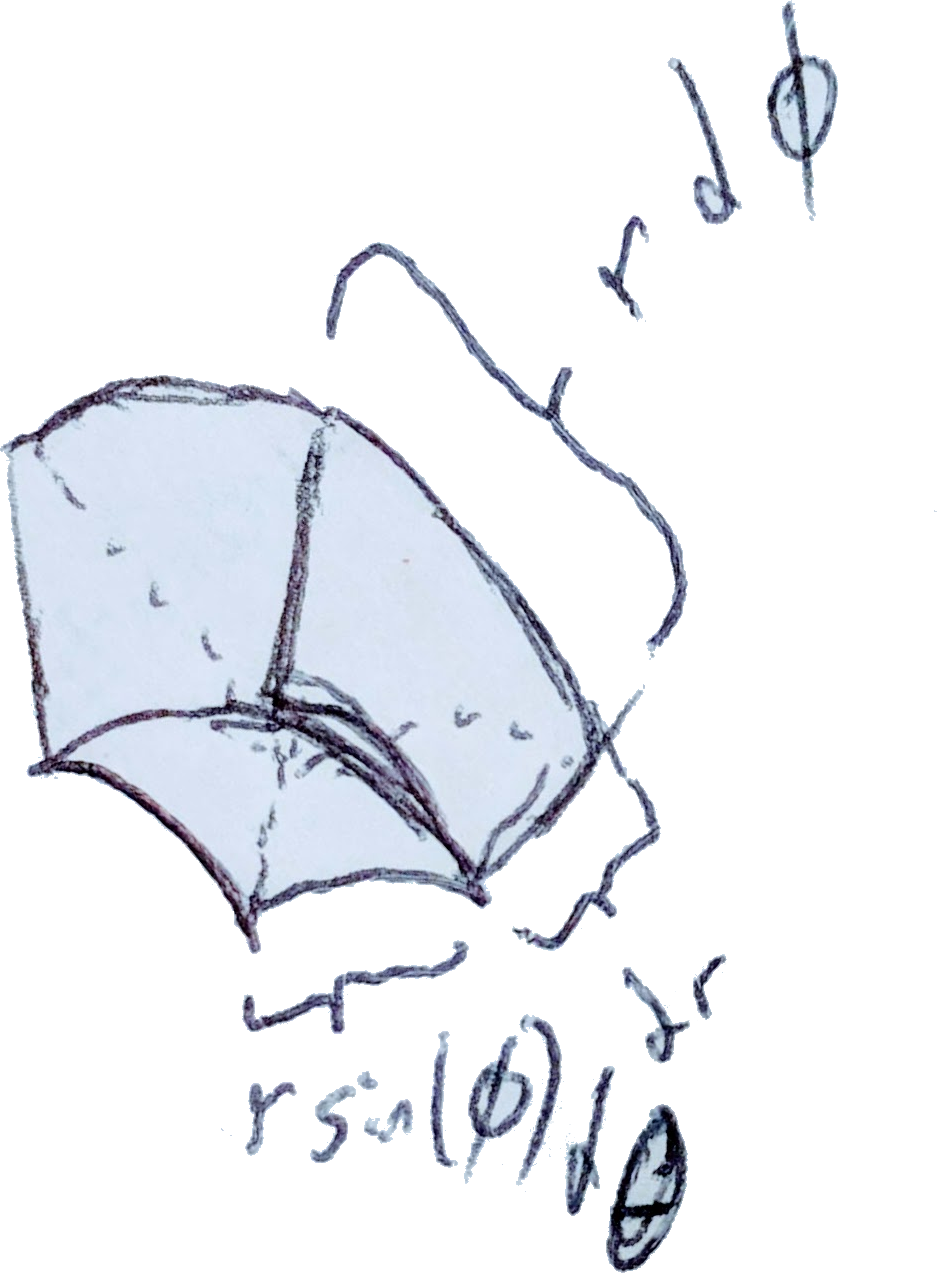
\includegraphics[width=100px]{mech222/worksheet_2b_spherical_diff_elem.png}
  \caption{Spherical coordinates differential area element}
\end{figure*}

Note that in general, we can use the Jacobian of the transformation to compute the differential element for any reasonable coordinate system.
\section*{Example}
Compute the integral of $f(x, y, z) = e^{x^2} x y z^2$ over the domain $D = \set{1 < x^2 + y^2 < 4, 0 < z < 3}$.

First, we note that we have a torus (donut) which is easily representable in polar coordinates which was then extruded into the $z$ direction.
Then it makes sense to work in cylindrical coordinates coordinates.

Converting our function to cylindrical coordinates, we have $\hat{f}(r, \theta, z) = e^{r^2 \cos^2(\theta)} r^2 \cos(\theta) \sin(\theta) z^2$.
Then converting our domain, we have $D = \set{1 < r < 2, 0 < \theta < 2 \pi, 0 < z < 3}$.

Our integral is then
\begin{equation*}
  \int_{z = 0}^{3} \int_{\theta = 0}^{2 \pi} \int_{r = 1}^{2} e^{r^2 \cos^2(\theta)} r^3 \cos(\theta) \sin(\theta) z^2 \dr \dd{\theta} \dz
\end{equation*}
Notice that applying Fubini's theorem to integrate $\theta$ before we integrate $r$ will make the integral easier by cancelling some of the $r$ terms.
Then substituting $u = \cos^2(\theta)$, $\dd{u} = -2 \cos(\theta) \sin(\theta)$ gives
\begin{align*}
  \int_{z = 0}^{3} & \int_{r = 1}^{2} \int_{\theta = 0}^{2 \pi} e^{r^2 \cos^2(\theta)} r^3 \cos(\theta) \sin(\theta) z^2 \dd{\theta} \dr \dz\\
  & = \int_{z = 0}^{3} \int_{r = 1}^{2} \int_{u = 1}^{1} -\frac{1}{2} e^{r^2 u} r^3 z^2 \dd{u} \dr \dz\\
  & = \int_{z = 0}^{3} \int_{r = 1}^{2} 0 \dr \dz = 0
\end{align*}
\section*{Problems}
For the following problems, draw the domains of integration, choose a coordinate system to integrate them in,
label the bounds for the variables of integration, and finally compute the integral
\begin{enumerate}
\item Compute the volume of a ball of radius $R$.\\
  \newline
  \newline
  \newline
  \newline
  \newline
  \newline
  \newline
\item Integrate $f(x, y, z) = x^2 + y^2$ over the intersection of the cone with $\phi = \frac{\pi}{4}$ and the unit sphere.\\
  \newline
  \newline
  \newline
  \newline
  \newline
  \newline
  \newline
\item Integrate $f(x, y, z) = x$ over the volume enclosed by $z = x^2 + y^2$ and $z = 2$.\\
  \newline
  \newline
  \newline
  \newline
  \newline
  \newline
  \newline
  \newline
\item Integrate $f(r, \theta, z) = r$ over $D = \set{1 < r < 3, 0 < \theta < 2 \pi, -\sqrt{1 - (r - 2)^2} < z < \sqrt{1 - (r - 2)^2}}$.\\
  \newline
  \newline
  \newline
  \newline
  \newline
  \newline
  \newline
  \newline
  \newline
  \newline
  \newline
\item Integrate $f(x, y, z) = x$ over the volume enclosed by $z = x^2 + y^2$ and $z = 2$.\\
  \newpage
\item Compute the center of mass of a cone with uniform density $\rho$ and boundaries $z = \sqrt{x^2 + y^2}$ and $z = 5$.\\
  \newline
  \newline
  \newline
  \newline
  \newline
  \newline
  \newline
  \newline
  \newline
  \newline
  \newline
  \newline
  \newline
  \newline
  \newline
  \newline
  \newline
  \newline
  \newline
  \newline
\item Compute moment of inertia for a hollow sphere with inner radius $r_1$ and outer radius $r_2$, with uniform density $\rho$.\\
  \newline
  \newline
  \newline
  \newline
  \newline
  \newline
  \newline
  \newline
  \newline
\end{enumerate}
\end{document}

